\subsection{File organization}\label{subsec:file-organization}
%\begin{center}
%    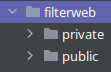
\includegraphics[scale=0.6]{web_main_folder}
%\end{center}
\begin{flushleft}
    In the main folder we can find the next directories:
        \begin{itemize}
            \item public
            \begin{itemize}
                \item In this directory is stored the files available to the user.
            \end{itemize}
            \item private
            \begin{itemize}
                \item In this directory will be stored the files that the user shouldn't have access.
            \end{itemize}
        \end{itemize}
\end{flushleft}

\newpage
\subsection{Public Directory Content}\label{subsec:public-directory-content}

\begin{flushleft}
    Point out that the content of the folder is named .index, to make it more visually appealing, yet this could be
    easily avoided by configuring Nginx, all the php files could follow this structure, it's just a matter of investing
    5 minutes (as much) in doing it.
\end{flushleft}
\begin{center}
    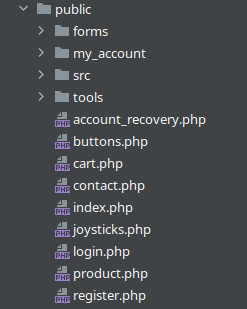
\includegraphics[scale=0.85]{web_public_directory}
\end{center}
In the public folder we can find the next directories:
\begin{itemize}
    \item forms
    \begin{itemize}
        \item Forms used to store the \textbf{API} entry points, used by the client.
    \end{itemize}
    \item my\_account
    \begin{itemize}
        \item Public pages that the user can access in order to manage its account.
    \end{itemize}
    \item tools
    \begin{itemize}
        \item Pages that fulfill a specific function and are often used.
    \end{itemize}
    \item src
    \begin{itemize}
        \item Used to store files that the user might require, mainly used to store:
        \begin{itemize}
            \item Images
            \item JavaScript
            \item Favicon
        \end{itemize}
    \end{itemize}
\end{itemize}
\newpage

\subsection{Private Directory Content}\label{subsec:private-directory-content}
\begin{flushleft}
    \textit{*The file \textbf{global\_vars.php} should be renamed "manager.php" or something like it in the future and
    be moved to the "libraries" folder.}
\end{flushleft}
\begin{center}
    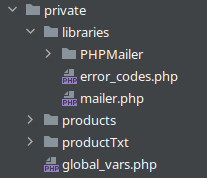
\includegraphics[scale=1]{web_public_private}
\end{center}
\begin{flushleft}
    In the private folder we can find the next directories:
\end{flushleft}
\begin{itemize}
    \item Used to store files that the user might require, mainly used to store:
    \begin{itemize}
        \item libraries directory
        \begin{itemize}
            \item Contains the libraries of:
            \begin{itemize}
                \item PHPMailer
                \item Error\_Codes
            \end{itemize}
        \end{itemize}
        \item Products folders
        \begin{itemize}
            \item Used to store information about products in order to showcase it in the demo, this could be easily
            replaced by importing the values to the database.
        \end{itemize}
    \end{itemize}
\end{itemize}

\subsection{Code Structure}\label{subsec:code-structure}

\begin{flushleft}
    Depending of the function of the file, the structure might vary, so far we can find 3 general structures:
    \begin{itemize}
        \item Library/package
        \item Public page
        \item API
    \end{itemize}
\end{flushleft}
\newpage
\subsubsection[Library/package code structure]{Library/package code structure}
\begin{flushleft}
    Meanwhile there is no code structure, the files are built trying to keep together the related.
\end{flushleft}

\subsubsection[Public page code structure]{Public page code structure}
\begin{flushleft}
    In this case we have a structure, yet, if it's necessary, the structure might vary according to the needs.
\end{flushleft}
\begin{flushleft}
\begin{lstlisting}[language=php,label={lst:php_page_structure}]
<?php
    require_once(global_vars.php);
    $global_vars = new page_vars();
    $global_vars->return_header();
    /* Print/do stuff */
    $global_vars->return_footer();
?>
\end{lstlisting}
\end{flushleft}

\newpage
\subsubsection[API code structure]{API code structure}
\begin{flushleft}
    The idea behind its structure, is attempt to do something, and in case of going wrong raises an Exception, then format a class that will be used as json output.
\end{flushleft}
\lstinputlisting[language=php,label={lst:php_api_structure}]{../config/filterweb/public/forms/account_management/add_shipping_address/index.php}

\newpage
\subsubsection[Main Class listing]{Class listing}

\begin{flushleft}
    The current main classes created are:
    \begin{itemize}
        \item json\_response
        \begin{itemize}
                \item Used to store the status from the API call, and return its values to the client.
        \end{itemize}
    \end{itemize}
    \begin{itemize}
        \item page\_vars
        \begin{itemize}
            \item Mainly used to store variables to be used among all the pages, and to return a footer and header
            that it's contents might vary depending on if the user it's logged or not.
            \item Also used to import the libraries if the corresponding function it's used, that way the code it's more consistent.
        \end{itemize}
    \end{itemize}
    \begin{itemize}
        \item Hotashi
        \begin{itemize}
            \item Responsible of getting the user cookies, posts, gets and validate its values, capable of rising errors if needed.
            \item Has some functions that make use of the class \textbf{db\_manager}, for example has a function that checks if the user session token is valid.
        \end{itemize}
    \end{itemize}
    \begin{itemize}
        \item db\_user
        \begin{itemize}
            \item Each entry stores information about the connection to the database, which includes the username, password, host among other data.
            \item Extends to \textbf{db\_user\_contact\_manager} and \textbf{db\_user\_shop\_manager}
        \end{itemize}
    \end{itemize}
    \begin{itemize}
        \item db\_manager
        \begin{itemize}
            \item Stores functions that contain calls to the database, also, \textbf{\_\_on\_construct} makes use of the \textbf{db\_user}  class to generate a PDO connection.
            \item Extends to \textbf{contact\_db\_manager} and \textbf{shop\_db\_manager}
            \item \begin{flushleft}
                An example of function that requires a PDO usage might be:
                \begin{lstlisting}[language=php,label={lst:php_pdo_query_example}]
public function add_shipping_address(hotashi $hotashi){
try {
    $stmt = $this->dbconn->prepare(query: 'call proc_add_shipping_address_from_stoken(?,?,?,?,?,?,?);');
    $stmt->execute(array($hotashi->stoken,$hotashi->sa_country,$hotashi->sa_city,$hotashi->sa_pcode,$hotashi->sa_add1,$hotashi->sa_add2,$hotashi->sa_add3));
}
catch (PDOException $e){
    $this->error_manager->pg_error_handler($e->getCode());
}
}
                \end{lstlisting}
            \end{flushleft}
        \end{itemize}
        \item
    \end{itemize}
    \begin{itemize}
        \item a
        \begin{itemize}
            \item
        \end{itemize}
    \end{itemize}
\end{flushleft}